\section{Results}

\subsection{Technical Benchmarking}

The technical benchmarking helped us to gain an overview of the overall performance of the system created. In the test run evaluated the following metrics were achieved:

Tool selection:
298+191 out of 609 times the correct tool was identified
56+64 out of 609 times the wrong tool was identified

Option matches for queries where the correct tool was determined:
72 out of 298 times all the required options were matched successfully without error
152 out of 298 times at least one of the required options was matched (on average 50.11\% of options required were included)
74 out of 298 times non of the required options were suggested.

for the queries with 100\% option recall the number of suggested options was of by an RSF of 1.67
For the queries with 50.11\% recall it was 1.68
for 0\% it was 1.64

Resolution failures:

out of 255 resolution failures 64 had teh wrong tool selected and 191 had the right tool but conflicting options

When the wrong tool was picked the command retrieval failed in 64 out of 64+56 cases
When the right tool was picked the command retrieval failed in 191 out of 191+298 cases


Command Execution Time (ms):
Average: 563.21 ms
Minimum (Fastest Query): 486.53 ms
Maximum (Slowest Query): 1570.54 ms
Slow Runs (>1000ms): 5 out of 609 (0.82\% of test set)

Peak Memory Usage (HWM / RSS):
Average: 674425.00 KB (658.62 MB)
Minimum (Lowest memory footprint): 663108.00 KB (647.57 MB)
Maximum (Highest memory footprint): 688676.00 KB (672.54 MB)


SSD runs in ZFS pool in proxmox, For performance:
zfs set sync=disabled rpool/data/vm-500-disk-1

\FloatBarrier

% ====================================================================
% GROUP A: Tool Selection Accuracy (Chart 1 & Chart 4 side-by-side)
% ====================================================================
\begin{figure}[htbp]
\centering
\begin{minipage}{0.48\textwidth}
  \centering
  \begin{tikzpicture}[scale=0.9]
    % Segment 1: Correct Tool (80.3%)
    \draw[fill=primaryblue] (0,0) -- (0:2) arc (0:289:2) -- cycle;
    % Segment 2: Wrong Tool (19.7%)
    \draw[fill=primaryorange] (0,0) -- (289:2) arc (289:360:2) -- cycle;
  \end{tikzpicture}
  \vspace{0.3cm}
  
  \small
  \begin{tabular}{llcc}
    \textcolor{primaryblue}{\rule{1.2ex}{1.2ex}} & Correct Tool & 489 & (80.3\%) \\
    \textcolor{primaryorange}{\rule{1.2ex}{1.2ex}} & Wrong Tool & 120 & (19.7\%) \\
  \end{tabular}
  \vspace{0.2cm}
  \caption{Overall Tool Selection Accuracy ($N=609$).}
  \label{fig:overall_tool_accuracy}
\end{minipage}
\hfill
\begin{minipage}{0.48\textwidth}
  \centering
  \begin{tikzpicture}[scale=0.9]
    % Segment 1: Correct Tool (74.9%)
    \draw[fill=primaryblue] (0,0) -- (0:2) arc (0:270:2) -- cycle;
    % Segment 2: Incorrect Tool (25.1%)
    \draw[fill=primaryorange] (0,0) -- (270:2) arc (270:360:2) -- cycle;
  \end{tikzpicture}
  \vspace{0.3cm}
  
  \small
  \begin{tabular}{llcc}
    \textcolor{primaryblue}{\rule{1.2ex}{1.2ex}} & Correct Tool & 191 & (74.9\%) \\
    \textcolor{primaryorange}{\rule{1.2ex}{1.2ex}} & Incorrect Tool & 64 & (25.1\%) \\
  \end{tabular}
  \vspace{0.2cm}
  \caption{Tool Selection Accuracy in Failures ($N_{\text{errors}}=255$).}
  \label{fig:failures_tool_accuracy}
\end{minipage}
\end{figure}

% ====================================================================
% GROUP B: Option Recall and Over-generation (Chart 2 & Chart 3 side-by-side)
% ====================================================================
\begin{figure}[htbp]
\centering
\begin{minipage}{0.48\textwidth}
  \centering
  \begin{tikzpicture}[scale=0.9]
    % Segment 1: Fully Correct (24.2%)
    \draw[fill=primarygreen] (0,0) -- (0:2) arc (0:87:2) -- cycle;
    % Segment 2: Partially Correct (51.0%)
    \draw[fill=primaryblue] (0,0) -- (87:2) arc (87:271:2) -- cycle;
    % Segment 3: Non-Correct (24.8%)
    \draw[fill=primaryorange] (0,0) -- (271:2) arc (271:360:2) -- cycle;
  \end{tikzpicture}
  \vspace{0.3cm}
  
  \small
  \begin{tabular}{llcc}
    \textcolor{primarygreen}{\rule{1.2ex}{1.2ex}} & Fully Correct & 72 & (24.2\%) \\
    \textcolor{primaryblue}{\rule{1.2ex}{1.2ex}} & Partially Correct & 152 & (51.0\%) \\
    \textcolor{primaryorange}{\rule{1.2ex}{1.2ex}} & Non-Correct & 74 & (24.8\%) \\
  \end{tabular}
  \vspace{0.2cm}
  \caption{Option Match Quality ($N_{\text{correct}} = 298$).}
  \label{fig:option_match_quality}
\end{minipage}
\hfill
\begin{minipage}{0.48\textwidth}
  \centering
  \begin{tikzpicture}[scale=0.85]
  \begin{axis}[
      ybar,
      enlargelimits=0.15,
      ylabel={Symmetric Count Error (RSF)},
      symbolic x coords={Fully, Partially, None},
      xtick=data,
      nodes near coords,
      nodes near coords align={vertical},
      ymin=1.0, ymax=2.0,
      width=6.5cm, height=5.5cm,
  ]
  \addplot[fill=primaryblue] coordinates {(Fully,1.67) (Partially,1.68) (None,1.64)};
  \end{axis}
  \end{tikzpicture}
  \caption{Symmetric Count Error (RSF) by Subcategory (1.00 is perfect).}
  \label{fig:rsf_by_subcategory}
\end{minipage}
\end{figure}

% ====================================================================
% GROUP C: Failure Resolution & Error Types (Chart 5 & Chart 6 side-by-side)
% ====================================================================
\begin{figure}[htbp]
\centering
\begin{minipage}{0.48\textwidth}
  \centering
  \begin{tikzpicture}[scale=0.85]
  \begin{axis}[
      ybar,
      bar width=10pt,
      ylabel={Number of Queries},
      symbolic x coords={Right, Wrong},
      xtick=data,
      nodes near coords,
      nodes near coords align={vertical},
      legend style={at={(0.5,-0.25)}, anchor=north, legend columns=-1},
      width=6.5cm, height=5.5cm,
  ]
  \addplot[fill=primarygreen] coordinates {(Right,298) (Wrong,56)};
  \addplot[fill=primaryred] coordinates {(Right,191) (Wrong,64)};
  \legend{Success, Fail}
  \end{axis}
  \end{tikzpicture}
  \caption{Resolution Status by Tool Correctness. Right = Correct Tool, Wrong = Wrong Tool.}
  \label{fig:resolution_by_tool}
\end{minipage}
\hfill
\begin{minipage}{0.48\textwidth}
  \centering
  \begin{tikzpicture}[scale=0.85]
  \begin{axis}[
      ybar,
      bar width=8pt,
      ylabel={Number of Queries},
      symbolic x coords={cp, mv, ops},
      xtick=data,
      nodes near coords,
      nodes near coords align={vertical},
      legend style={at={(0.5,-0.25)}, anchor=north, legend columns=-1},
      width=6.5cm, height=5.5cm,
  ]
  \addplot[fill=primaryred] coordinates {(cp,16) (mv,30) (ops,10)};
  \addplot[fill=primaryorange] coordinates {(cp,35) (mv,21) (ops,0)};
  \legend{Over, Missed}
  \end{axis}
  \end{tikzpicture}
  \caption{Category-specific Errors: Over-generation (Over) vs. Missed Expected (Missed).}
  \label{fig:errors_by_category}
\end{minipage}
\end{figure}

% ====================================================================
% GROUP D: Global Dataset Breakdowns (Chart 8 & Chart 9 side-by-side)
% ====================================================================
\begin{figure}[htbp]
\centering
\begin{minipage}{0.48\textwidth}
  \centering
  \begin{tikzpicture}[scale=0.9]
    % Segment 1: Succeeded & Correct Tool (48.9%)
    \draw[fill=primarygreen] (0,0) -- (0:2) arc (0:176.1:2) -- cycle;
    % Segment 2: Succeeded & Wrong Tool (9.2%)
    \draw[fill=primaryblue] (0,0) -- (176.1:2) arc (176.1:209.2:2) -- cycle;
    % Segment 3: Failed & Correct Tool (31.4%)
    \draw[fill=primaryorange] (0,0) -- (209.2:2) arc (209.2:322.1:2) -- cycle;
    % Segment 4: Failed & Wrong Tool (10.5%)
    \draw[fill=primaryred] (0,0) -- (322.1:2) arc (322.1:360:2) -- cycle;
  \end{tikzpicture}
  \vspace{0.3cm}
  
  \small
  \begin{tabular}{llcc}
    \textcolor{primarygreen}{\rule{1.2ex}{1.2ex}} & Succeeded \& Correct Tool & 298 & (48.9\%) \\
    \textcolor{primaryblue}{\rule{1.2ex}{1.2ex}} & Succeeded \& Wrong Tool & 56 & (9.2\%) \\
    \textcolor{primaryorange}{\rule{1.2ex}{1.2ex}} & Failed \& Correct Tool & 191 & (31.4\%) \\
    \textcolor{primaryred}{\rule{1.2ex}{1.2ex}} & Failed \& Wrong Tool & 64 & (10.5\%) \\
  \end{tabular}
  \vspace{0.2cm}
  \caption{Overall dataset breakdown ($N=609$).}
  \label{fig:overall_breakdown}
\end{minipage}
\hfill
\begin{minipage}{0.48\textwidth}
  \centering
  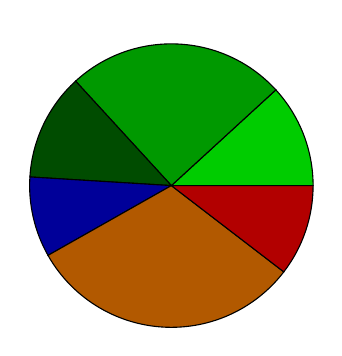
\begin{tikzpicture}[scale=0.9]
    % Segment 1: Fully Correct (11.8%)
    \draw[fill=green!80!black] (0,0) -- (0:2) arc (0:42.5:2) -- cycle;
    % Segment 2: Partially Correct (25.0%)
    \draw[fill=green!60!black] (0,0) -- (42.5:2) arc (42.5:132.5:2) -- cycle;
    % Segment 3: Non-Correct (12.2%)
    \draw[fill=green!30!black] (0,0) -- (132.5:2) arc (132.5:176.5:2) -- cycle;
    % Segment 4: Succeeded & Wrong (9.2%)
    \draw[fill=blue!60!black] (0,0) -- (176.5:2) arc (176.5:209.5:2) -- cycle;
    % Segment 5: Failed & Correct (31.4%)
    \draw[fill=orange!70!black] (0,0) -- (209.5:2) arc (209.5:322.5:2) -- cycle;
    % Segment 6: Failed & Wrong (10.5%)
    \draw[fill=red!70!black] (0,0) -- (322.5:2) arc (322.5:360:2) -- cycle;
  \end{tikzpicture}
  \vspace{0.3cm}
  
  \scriptsize
  \begin{tabular}{llcc}
    \textcolor{green!80!black}{\rule{1.2ex}{1.2ex}} & Fully Correct (100\% match) & 72 & (11.8\%) \\
    \textcolor{green!60!black}{\rule{1.2ex}{1.2ex}} & Partially Correct (1-99\% match) & 152 & (25.0\%) \\
    \textcolor{green!30!black}{\rule{1.2ex}{1.2ex}} & Non-Correct (0\% match) & 74 & (12.2\%) \\
    \textcolor{blue!60!black}{\rule{1.2ex}{1.2ex}} & Succeeded \& Wrong Tool & 56 & (9.2\%) \\
    \textcolor{orange!70!black}{\rule{1.2ex}{1.2ex}} & Failed \& Correct Tool & 191 & (31.4\%) \\
    \textcolor{red!70!black}{\rule{1.2ex}{1.2ex}} & Failed \& Wrong Tool & 64 & (10.5\%) \\
  \end{tabular}
  \vspace{0.2cm}
  \caption{Granular 6-category classification split ($N=609$).}
  \label{fig:detailed_breakdown}
\end{minipage}
\end{figure}

% ====================================================================
% STANDALONE: CHART 7: Command Execution Time Latency Bins (Bar Chart)
% ====================================================================
\begin{figure}[htbp]
\centering
\begin{tikzpicture}
\begin{axis}[
    ybar,
    bar width=20pt,
    ylabel={Number of Queries},
    symbolic x coords={Runs <= 1000ms, Runs > 1000ms},
    xtick=data,
    nodes near coords,
    nodes near coords align={vertical},
    ymin=0, ymax=650,
    width=8cm, height=6cm,
]
\addplot[fill=primaryblue] coordinates {(Runs <= 1000ms,604) (Runs > 1000ms,5)};
\end{axis}
\end{tikzpicture}
\caption{Command Execution Time Latency Bins ($N=609$). 604 runs completed in under 1 second, while only 5 exceeded 1000ms.}
\label{fig:latency_bins}
\end{figure}

\FloatBarrier

\subsection{User Study}